\documentclass[UTF8,a4paper]{ctexart}
%\usepackage[UTF8]{ctex}
\usepackage{graphicx}
\usepackage{url}
\usepackage{geometry}
\geometry{a4paper,scale=0.8}
\usepackage{setspace}
\setstretch{1.6}
\usepackage{listings}
\usepackage{xcolor}
\lstset{ 
  language=Python,  % 设置语言
  backgroundcolor=\color{lightgray},   % 背景颜色
  basicstyle=\ttfamily,    % 基本字体样式
  keywordstyle=\color{blue}, % 关键字颜色
  commentstyle=\color{gray}, % 注释颜色
  stringstyle=\color{red},   % 字符串颜色
  showspaces=false,          % 不显示空格
  showstringspaces=false,    % 字符串中的空格不显示
}

\begin{document}
\begin{sloppypar}


	\begin{center}
	
\includegraphics[width = 14cm]{picture/s1}

		\begin{fontsize}{60pt}{20pt}
			实验报告
		\end{fontsize}

		\bigskip
		\bigskip
		
		\begin{fontsize}{20pt}{20pt}
			\begin{flushright}
				—— 调试性能分析与元编程大杂烩及{\Huge pytorch}的学习
			\end{flushright}
		\end{fontsize}
		
		\bigskip
		\bigskip
		\bigskip
		\bigskip
		\bigskip
		\bigskip
		\bigskip
		\bigskip
		\bigskip
		\bigskip
		\bigskip
		\bigskip
		\bigskip
		\bigskip
		\bigskip
		\bigskip
		
		\begin{fontsize}{25pt}{20pt}

			学号:
			\underline{{\huge 23060021010}}
			\bigskip
			\bigskip
			\bigskip
			\bigskip

			姓名:
			\underline{郭晓伟}
			\bigskip
			\bigskip
			\bigskip
			\bigskip

			班级:
			\underline{{\Huge 23}级软件工程五八班}
				
		\end{fontsize}
	\end{center}
	\section{实验要求}
	\subsection{学习调试及性能分析}
	\subsection{初步了解元编程,学习大杂烩里的内容}
	\subsection{初步学会pytorch的使用}
	\subsection{完成与学习内容相关的4个课堂练习与20个实例}

			\bigskip
			\bigskip
			\bigskip
			\bigskip

	\section{实验内容}
	\subsection{调试代码}
	\subsubsection{打印调试法和日志:\\1.打印调试法:最简单的调试方式,通过在代码中的关键位置打印变量值、状态信息,来了解程序执行流程和错误原因。适合初期排查问题,缺点是容易让代码凌乱。\\2.日志(Logging):比打印更为系统化的调试方法,允许根据不同的严重性(如DEBUG、INFO、WARNING、ERROR等)记录程序执行的详细信息。日志可以持久化保存,方便回溯问题。\\3.Python的logging模块是常用的日志库,允许开发者根据需求动态设置日志的级别、格式、输出目的(如文件、控制台)。}
	\subsubsection{第三方日志系统:\\1.Logstash、Fluentd:这些系统用于收集、处理和存储日志。它们允许从多个来源收集日志,并支持过滤、转换和发送日志到存储系统。\\2.ELK Stack(Elasticsearch, Logstash, Kibana):一个流行的日志分析平台,提供了日志聚合、搜索和可视化功能。Kibana可帮助开发者直观地分析日志信息,发现异常模式。}
	\subsubsection{调试器:提供实时控制代码执行的工具,允许设置断点、查看和修改运行时变量、逐步执行代码等。\\GDB:一个常用的C/C++调试器,允许检查代码的内存、寄存器状态等。\\PDB:Python的标准调试器,允许在交互式命令行中调试Python代码。\\IDE集成调试器:大部分IDE(如PyCharm、VSCode)都有内置调试器,支持图形化界面下的断点、变量查看等功能。}
	\subsubsection{静态分析:通过分析源代码而不执行程序来发现代码中的错误、潜在问题或优化机会。\\Pylint、Flake8:Python中的静态分析工具,可以检查代码风格、潜在错误、复杂度等问题。\\Clang Static Analyzer:C/C++代码的静态分析工具,可以检测内存泄漏、未定义行为等问题。\\SonarQube:支持多种语言的静态代码分析平台,集成了代码质量检测和技术债务管理。}
	
	\newpage
	
	\subsection{性能分析}
	\subsubsection{手动计时:通过记录开始和结束时间来测量某个代码片段的运行时间。\\1.Python的time模块和timeit库都可以帮助精确测量代码段的执行时间。\\2.timeit特别适用于评估小代码段的性能,它自动管理计时和重复运行测试。}
	\subsubsection{性能分析工具Profiling:通过分析程序运行过程中的资源使用情况(如CPU、内存)来找出性能瓶颈。\\cProfile:Python自带的性能分析工具,记录每个函数调用的次数和执行时间,帮助找出性能热点。\\Py-Spy:一个性能监控工具,不影响程序的正常运行,适合对生产环境中的Python应用进行性能分析。\\Valgrind:用于C/C++程序的性能分析工具,可以检测内存泄漏、缓存未命中等问题。}
	\subsubsection{事件驱动的性能分析:一些性能问题只能在特定事件发生时暴露。通过记录系统或程序中的事件流,可以找到特定的性能瓶颈。\\性能可视化:通过图形化工具展示性能分析的结果,更容易找出性能瓶颈。\\资源监控:监控程序运行时的CPU、内存、磁盘I/O、网络等资源的使用情况,帮助评估系统性能。}
	\subsubsection{通过这些调试和性能分析的方法与工具,可以全面分析代码质量、资源使用情况,从而提高系统的稳定性和效率。}
	
	\bigskip
	\bigskip
	\bigskip
	\bigskip
	
	\subsection{元编程}
	\subsubsection{元编程(Metaprogramming)通常被理解为编写能够操作或生成其他代码的代码,在本课中更多指的是开发流程中的自动化和管理,包括构建系统、代码测试以及依赖管理。这类元编程的目标是让开发流程更加高效、自动化,减少人工干预和重复劳动。}
	\subsubsection{构建系统的主要任务是将源代码转换为可执行程序或其他可交付的输出(如库、文档等)。它自动处理编译、链接、打包、测试和发布等流程,减少人为操作。\\关键功能:编译代码、管理依赖、任务自动化、增量构建\\常见的构建工具:Make、CMake、Maven等}
	\subsubsection{代码测试在软件开发过程中至关重要,它通过自动化的测试流程保证代码的正确性、健壮性和可维护性。元编程在测试中的主要作用是自动化测试的执行、结果收集、分析以及集成测试的管理。\\测试的类型:\\单元测试(Unit Testing):测试代码中的最小功能单位,通常是函数或类的测试。\\集成测试(Integration Testing):测试不同模块或服务之间的交互,确保它们能正确协同工作。\\端到端测试(End-to-End Testing):从用户视角出发,测试整个系统的功能,模拟用户的操作流程。\\回归测试(Regression Testing):在代码更新后,确保新增或修改的代码没有引入新的错误。}
	
	\newpage
	
	\subsubsection{依赖管理用于确保项目中的外部库、工具和其他依赖项被正确地下载、安装和使用。有效的依赖管理工具能避免依赖冲突、版本不一致等问题,并自动处理依赖的升级和发布。\\依赖管理的核心内容:依赖声明:开发者通过配置文件或声明语法描述项目所依赖的库及其版本。\\版本控制:依赖管理工具会根据依赖声明下载对应版本的库,并确保项目使用兼容的版本。\\依赖冲突解决:当不同依赖项之间存在版本冲突时,依赖管理工具会自动选择合适的版本或提供冲突解决方案。\\缓存与镜像:通过本地缓存或镜像服务器加速依赖的下载和安装过程。}
	
	\bigskip
	\bigskip
	\bigskip
	\bigskip
	
	\subsection{PyTorch}
	\subsubsection{PyTorch是一个由 Facebook AI Research (FAIR) 团队开发的开源深度学习框架,专注于灵活的模型定义、易用性和高效的自动求导系统。它在学术界和工业界广泛使用,特别是在计算机视觉、自然语言处理等领域。PyTorch 的核心特性包括动态计算图、GPU加速、自动微分,以及一个功能丰富的生态系统,涵盖从研究到生产的深度学习工作流。}
	\subsubsection{PyTorch的核心特性:\\1.动态计算图:PyTorch 使用动态计算图,即模型的计算图在每次前向传播时即时构建。这种方式称为“Define-by-Run”,允许用户根据输入数据动态修改模型结构,非常适合调试和灵活构建复杂的神经网络。\\2.自动微分:PyTorch 提供了强大的自动微分功能,支持通过后向传播自动计算梯度。这是通过 autograd 模块实现的,它会记录每个操作,构建计算图,并根据需要进行梯度计算。\\3.张量计算与GPU加速:PyTorch 的核心是对张量(Tensor)的高效操作,张量是多维数组,类似于 NumPy 中的 ndarray。PyTorch 的张量可以在 GPU 上加速执行,借助 GPU 的并行计算能力,大大提高深度学习模型的训练速度。}
	\subsubsection{PyTorch的基本组件:\\1.Tensor张量:张量是 PyTorch 的核心数据结构,它类似于 NumPy 的多维数组,但可以在 GPU 上执行高效的并行计算。张量的操作包括基本的数值运算、线性代数、矩阵运算等。\\2.神经网络:torch.nn 模块提供了构建神经网络的基本构件,如层(Layer)、损失函数(Loss Function)、激活函数(Activation Function)等。PyTorch 的模块化设计允许用户轻松构建、组合和训练复杂的神经网络模型。\\3.优化器:优化器模块负责更新模型的参数,以最小化损失函数。PyTorch 提供了多种优化算法的实现,如随机梯度下降(SGD)、Adam、RMSprop 等。}
	
	\graphicspath{{picture/}}

	\newpage
	
	\section{实验中遇到的问题与解决方法}
	\subsection{已安装Pytorch,却提示no moudle named ‘torch’}
	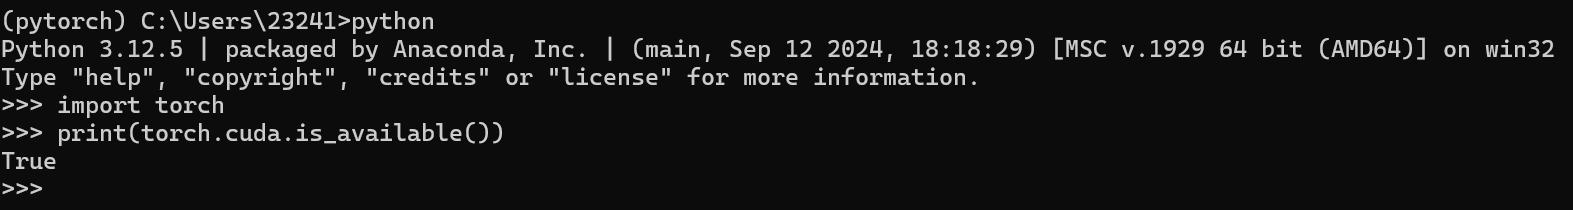
\includegraphics[width = 16cm]{q1}
	解决:用conda activate xxx 激活pytorch所在环境后再运行代码,即可解决,如图成功打印出true。
	\subsection{pycharm配置anaconda环境时找不到python.exe}
	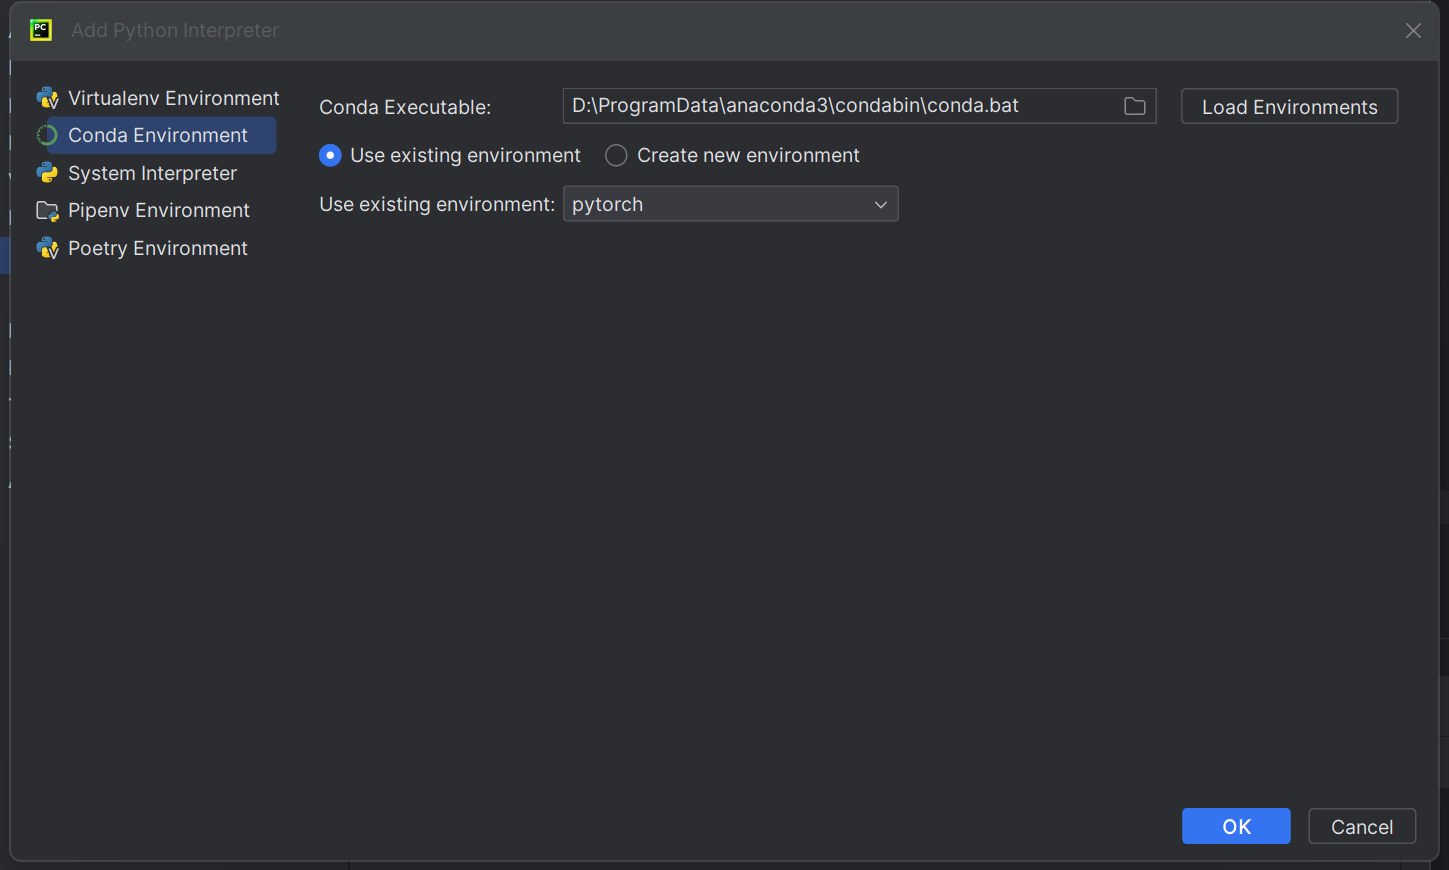
\includegraphics[width = 16cm]{q2}
	解决:这是由于pycharm版本过新,在路径中找到conda.bat文件,之后Load Environments,将会自动加载出存在的环境,就可以找到虚拟环境的解释器了,如图,pycharm中的Console成功输出true。
	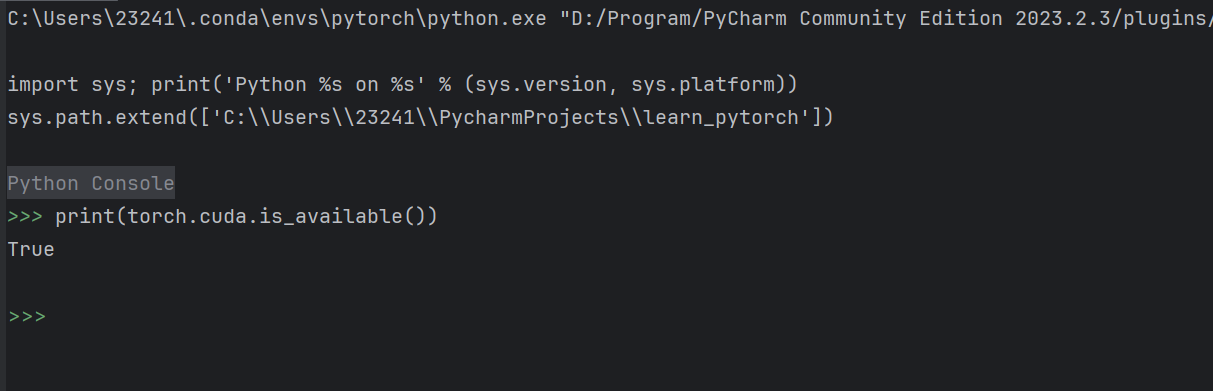
\includegraphics[width = 16cm]{q3}
	
	\newpage
	
	\section{实例练习}
	\subsection{向系统日志中写日志并读取}
	使用logger这个shell程序将日志加入到系统日志中,并使用journalctl输出日志,由于日志内容过多,使用grep hello 过滤

	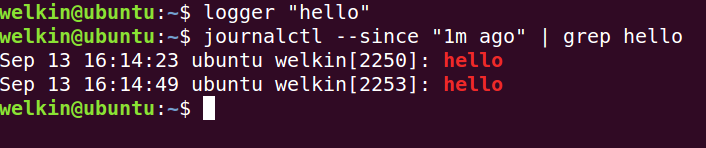
\includegraphics[width = 16cm]{1}
	
	\subsection{Python中使用日志记录调试}
	使用 Python 的 logging 模块代替 print() 进行更细致的调试。这种方式更灵活,日志可以保存到文件或通过不同的日志级别筛选输出,在复杂项目中尤为有用
	
	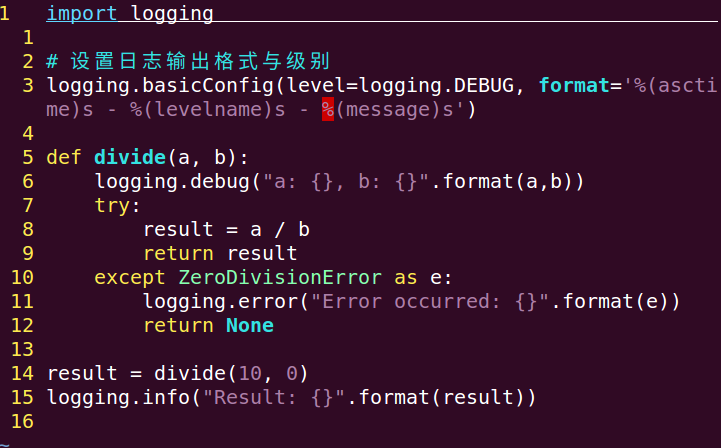
\includegraphics[width = 16cm]{21}
	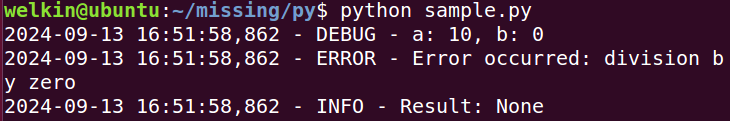
\includegraphics[width = 16cm]{22}
	
	\subsection{性能分析之手动计时}
	最简单的性能分析方法即手动计时,用于测量代码执行时间,代码如下
	\begin{lstlisting}
import time

start_time = time.time()

# 模拟耗时操作
result = sum(range(1000000))

end_time = time.time()
print(f"Execution time: {end_time - start_time} seconds")
	\end{lstlisting}
	
	\subsection{使用cProfile进行性能分析}
	cProfile 是 Python 内置的性能分析工具,可以用来分析程序的执行时间,找出最耗时的函数和代码路径。如图所示
	
	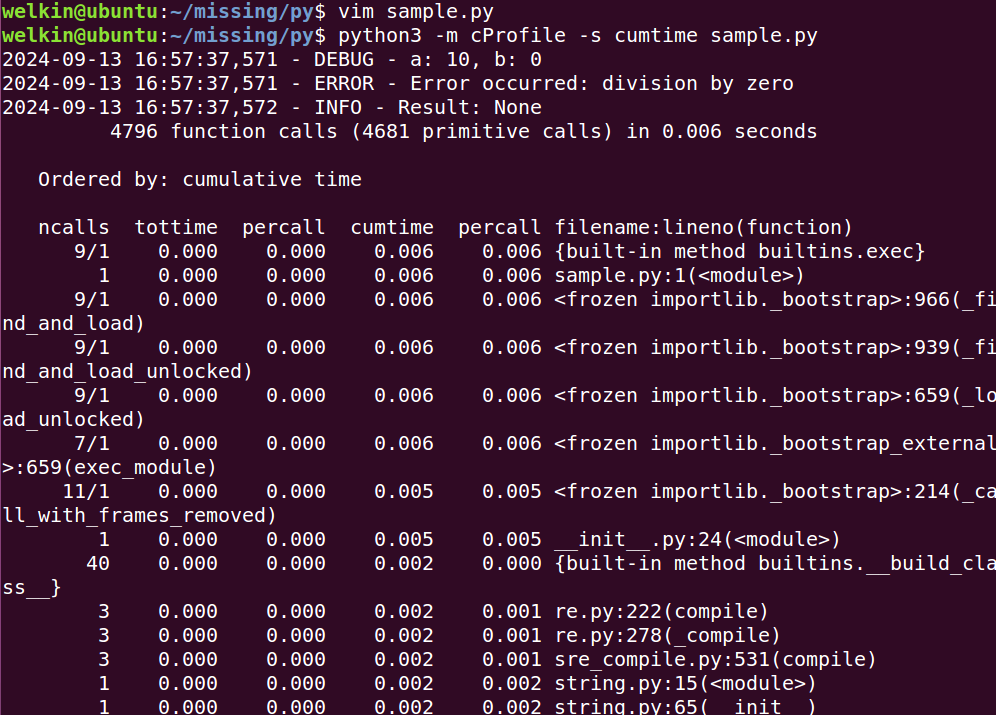
\includegraphics[width = 16cm]{4}
	
	\subsection{Markdown标题}
	
	
\includegraphics[width = 16cm]{51}
	
\includegraphics[width = 16cm]{52}
	
	\subsection{Markdown字体}

	
\includegraphics[width = 16cm]{61}
	
\includegraphics[width = 16cm]{62}
	
	\subsection{Markdown无序列表}

	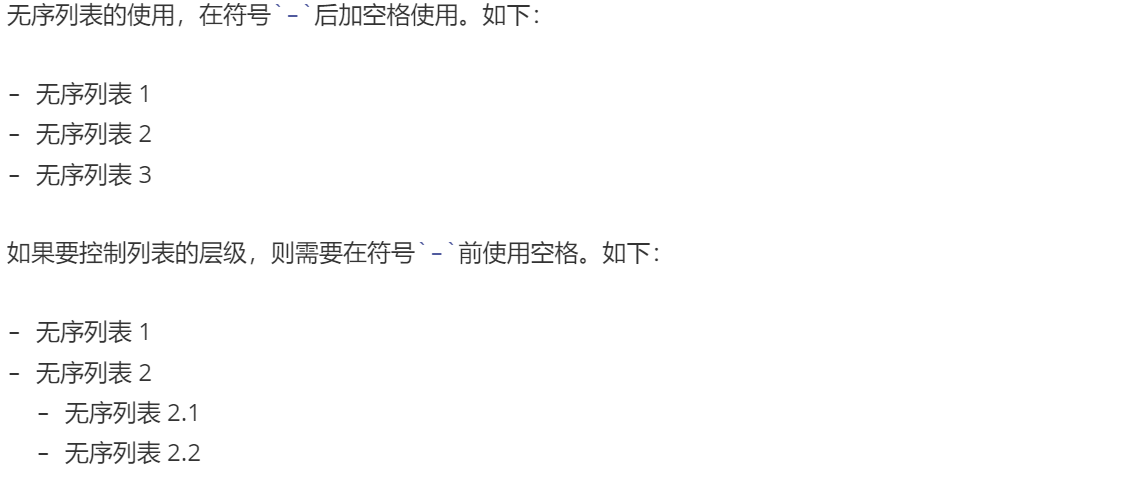
\includegraphics[width = 16cm]{71}
	
\includegraphics[width = 16cm]{72}
	
	\subsection{Markdown代码块}

	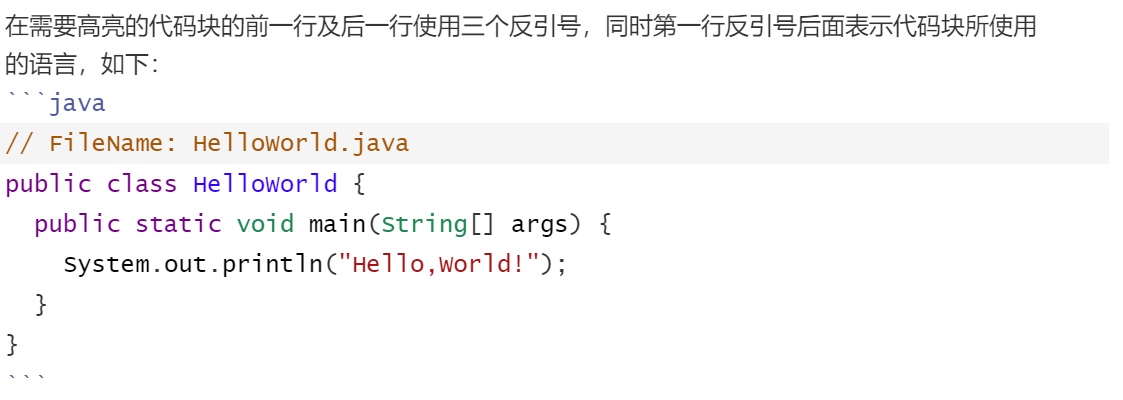
\includegraphics[width = 16cm]{81}
	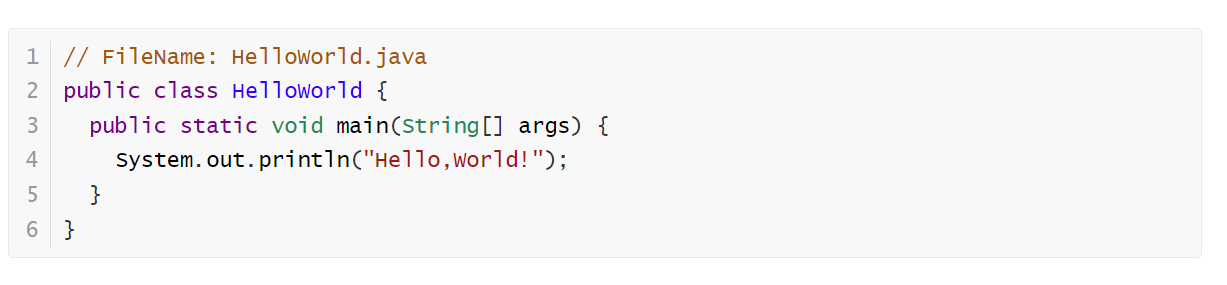
\includegraphics[width = 16cm]{82}
	
	\subsection{Markdown实现矩阵}

	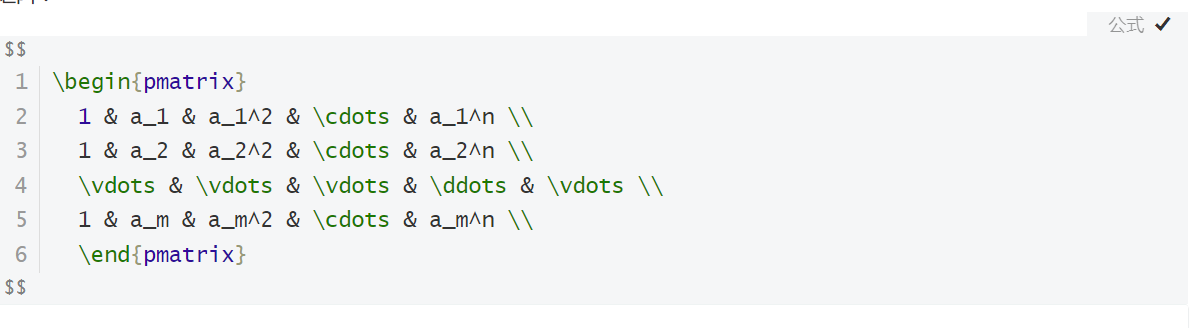
\includegraphics[width = 16cm]{91}
	
\includegraphics[width = 16cm]{92}
	
	
	\subsection{创建和操作张量}
	使用torch.tensor创建张量,并直接计算


	\begin{lstlisting}
import torch

# 创建两个张量
a = torch.tensor([[1.0, 2.0], [3.0, 4.0]])
b = torch.tensor([[5.0, 6.0], [7.0, 8.0]])

# 加法操作
c = a + b

# 逐元素乘法
d = a * b

print("a + b = \n", c)
print("a * b = \n", d)
	\end{lstlisting}
	
	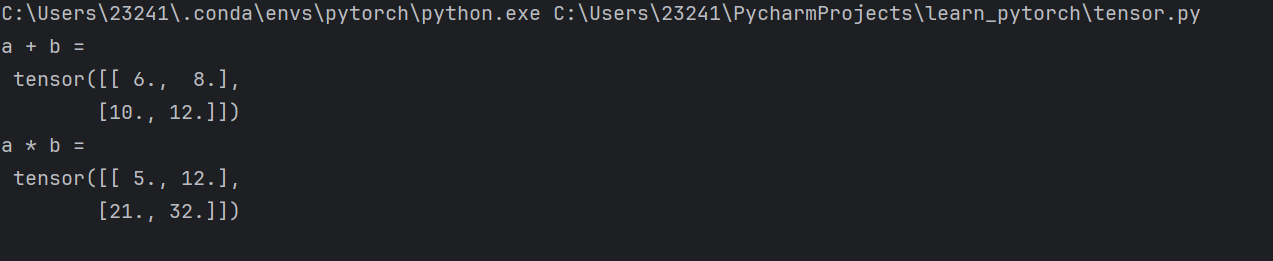
\includegraphics[width = 16cm]{10}
	
	
	\subsection{使用自动微分}
	requires\_grad=True,告诉 PyTorch 需要计算梯度,x可微分,y.backward()执行反向传播,计算 y 相对于 x 的梯度。
	\begin{lstlisting}
import torch

# 创建一个张量并启用自动求导
x = torch.tensor(2.0, requires_grad=True)

# 计算一个简单的函数
y = x ** 2 + 3 * x + 1

# 反向传播计算梯度
y.backward()

# 查看梯度
print(f"x的梯度: {x.grad}")
    \end{lstlisting}
	
	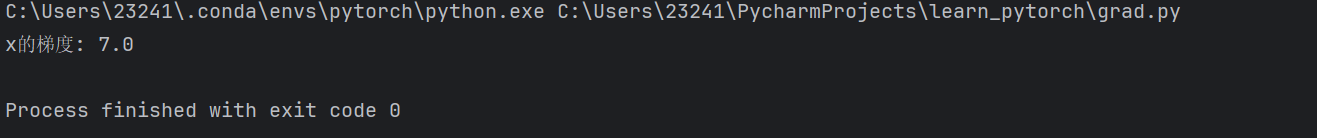
\includegraphics[width = 16cm]{11}
	
	
	\subsection{构建简单的线性模型}
	nn.Module为PyTorch中所有神经网络的基类,然后定义一个线性层,输入和输出维度均为1
\begin{lstlisting}
import torch
import torch.nn as nn

# 定义一个简单的线性模型
class LinearModel(nn.Module):
    def __init__(self):
        super(LinearModel, self).__init__()
        self.linear = nn.Linear(1, 1)

    def forward(self, x):
        return self.linear(x)

# 实例化模型
model = LinearModel()

\end{lstlisting}
	
	
	\subsection{训练一个简单的线性模型}
	使用一系列函数,并每500个epoch打印一次损失值
	\begin{lstlisting}
import torch
import torch.nn as nn
import torch.optim as optim

# 定义模型、损失函数和优化器
model = LinearModel()
criterion = nn.MSELoss()  # 均方误差损失函数
optimizer = optim.SGD(model.parameters(), lr=0.01)  # 随机梯度下降

# 生成一些随机数据
x_train = torch.randn(100, 1)
y_train = 3 * x_train + 2 + torch.randn(100, 1) * 0.1  # 模拟数据

# 训练模型
for epoch in range(500):
    optimizer.zero_grad()  # 清除上一步的梯度
    outputs = model(x_train)  # 前向传播
    loss = criterion(outputs, y_train)  # 计算损失
    loss.backward()  # 反向传播
    optimizer.step()  # 更新参数

    if (epoch + 1) % 100 == 0:
        print(f'Epoch [{epoch+1}/500], Loss: {loss.item():.4f}')
	\end{lstlisting}
	
	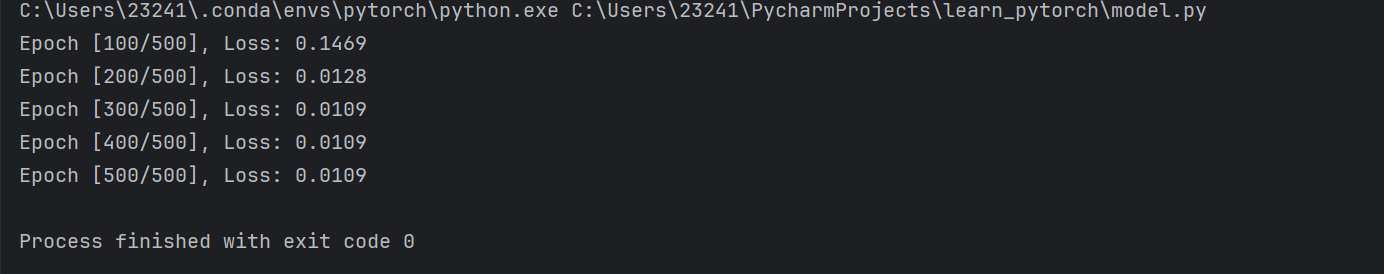
\includegraphics[width = 16cm]{13}
	
	\subsection{使用torch.nn.functional}
	torch.nn.functional: 提供一些常用的函数,如激活函数 relu 等。与 torch.nn 中的层不同,torch.nn.functional 不需要实例化
	\begin{lstlisting}
import torch
import torch.nn as nn
import torch.nn.functional as F

# 创建一个简单的模型
class SimpleNN(nn.Module):
    def __init__(self):
        super(SimpleNN, self).__init__()
        self.linear = nn.Linear(10, 2)

    def forward(self, x):
        x = self.linear(x)
        return F.relu(x)  # 使用 torch.nn.functional 中的激活函数

# 实例化模型并使用
model = SimpleNN()
x = torch.randn(1, 10)
output = model(x)
print(output)
    \end{lstlisting}
	
	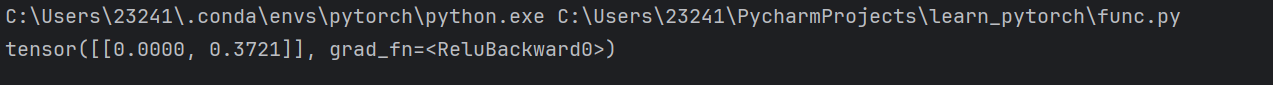
\includegraphics[width = 16cm]{14}


	\subsection{简单的线性回归}
	定义简单的线性回归模型,并使用随机梯度下降法来更新模型参数
	\begin{lstlisting}
import torch
import torch.nn as nn
import torch.optim as optim

# 定义线性回归模型
model = nn.Linear(1, 1)

# 定义损失函数和优化器
criterion = nn.MSELoss()
optimizer = optim.SGD(model.parameters(), lr=0.01)

# 生成一些随机数据
x_train = torch.randn(100, 1)
y_train = 5 * x_train + 3 + torch.randn(100, 1) * 0.5

# 训练模型
for epoch in range(300):
    optimizer.zero_grad()
    y_pred = model(x_train)
    loss = criterion(y_pred, y_train)
    loss.backward()
    optimizer.step()

    if (epoch + 1) % 50 == 0:
        print(f'Epoch [{epoch+1}/300], Loss: {loss.item():.4f}')
    \end{lstlisting}
	
	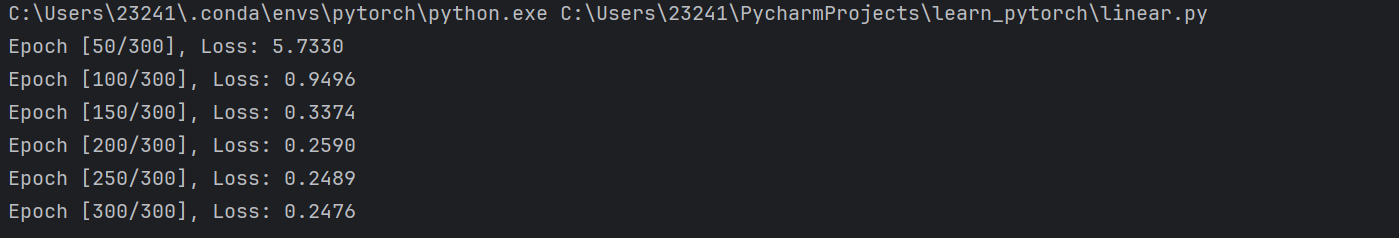
\includegraphics[width = 16cm]{15}
	
	\subsection{数据加载与批处理}
	TensorDataset将x\_data和y\_data组合成数据集,shuffle=True表示打乱数据顺序
	\begin{lstlisting}
import torch
from torch.utils.data import DataLoader, TensorDataset

# 创建张量数据
x_data = torch.randn(100, 1)
y_data = 3 * x_data + 2 + torch.randn(100, 1) * 0.1

# 创建 TensorDataset 和 DataLoader
dataset = TensorDataset(x_data, y_data)
dataloader = DataLoader(dataset, batch_size=10, shuffle=True)

# 遍历数据加载器
for inputs, targets in dataloader:
    print(inputs, targets)
    \end{lstlisting}
	
	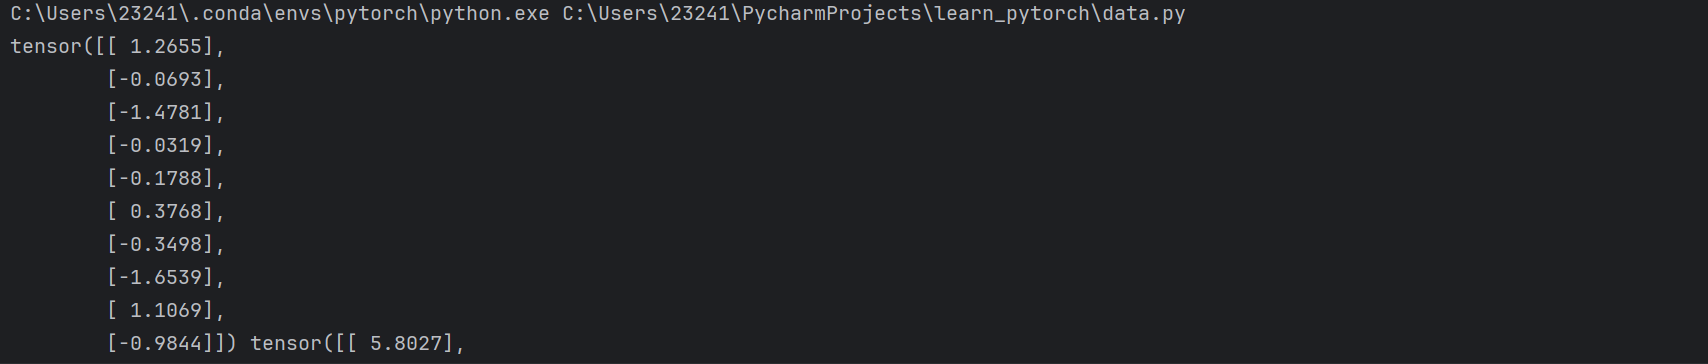
\includegraphics[width = 16cm]{16}
	
	\subsection{简单的逻辑回归(二分类)}
	逻辑回归模型,用于二分类问题,输出 0 或 1 的概率,并将线性输出转换为概率值
	\begin{lstlisting}
import torch
import torch.nn as nn
import torch.optim as optim

# 定义逻辑回归模型
class LogisticRegression(nn.Module):
    def __init__(self):
        super(LogisticRegression, self).__init__()
        self.linear = nn.Linear(2, 1)

    def forward(self, x):
        return torch.sigmoid(self.linear(x))

# 创建数据
x_train = torch.tensor([[1, 2], [2, 3], [3, 4], [4, 5]], dtype=torch.float32)
y_train = torch.tensor([[0], [0], [1], [1]], dtype=torch.float32)

# 实例化模型、损失函数和优化器
model = LogisticRegression()
criterion = nn.BCELoss()
optimizer = optim.SGD(model.parameters(), lr=0.01)

# 训练模型
for epoch in range(1000):
    optimizer.zero_grad()
    y_pred = model(x_train)
    loss = criterion(y_pred, y_train)
    loss.backward()
    optimizer.step()

    if (epoch + 1) % 200 == 0:
        print(f'Epoch [{epoch+1}/1000], Loss: {loss.item():.4f}')
    \end{lstlisting}
	
	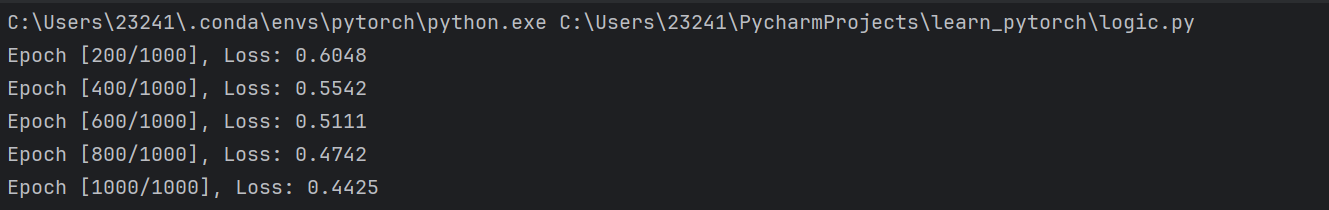
\includegraphics[width = 16cm]{17}
	
	\subsection{简单的多分类问题}
	多分类模型将输出3个类别的概率,torch.softmax用于将输出转化为概率分布
	\begin{lstlisting}
import torch
import torch.nn as nn
import torch.optim as optim

# 定义多分类模型
class MulticlassNN(nn.Module):
    def __init__(self):
        super(MulticlassNN, self).__init__()
        self.linear = nn.Linear(4, 3)

    def forward(self, x):
        return torch.softmax(self.linear(x), dim=1)

# 创建数据
x_train = torch.randn(10, 4)
y_train = torch.randint(0, 3, (10,))

# 实例化模型、损失函数和优化器
model = MulticlassNN()
criterion = nn.CrossEntropyLoss()
optimizer = optim.SGD(model.parameters(), lr=0.01)

# 训练模型
for epoch in range(500):
    optimizer.zero_grad()
    outputs = model(x_train)
    loss = criterion(outputs, y_train)
    loss.backward()
    optimizer.step()

    if (epoch + 1) % 100 == 0:
        print(f'Epoch [{epoch+1}/500], Loss: {loss.item():.4f}')
    \end{lstlisting}
	
	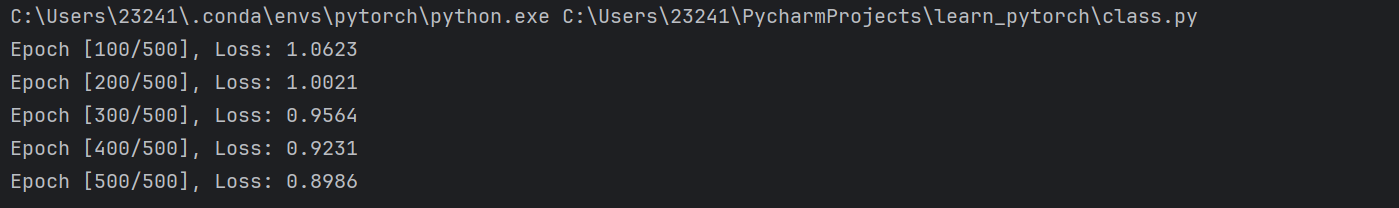
\includegraphics[width = 16cm]{18}
	
	\subsection{简易自定义神经网络层}
	创建一个自定义的神经网络层,该层包含一个可训练的权重参数
	\begin{lstlisting}
import torch
import torch.nn as nn

# 自定义简单的神经网络层
class CustomLayer(nn.Module):
    def __init__(self):
        super(CustomLayer, self).__init__()
        self.weight = nn.Parameter(torch.randn(1))

    def forward(self, x):
        return x * self.weight

# 使用自定义层
x = torch.randn(1, 10)
layer = CustomLayer()
output = layer(x)
print(output)
    \end{lstlisting}
	
	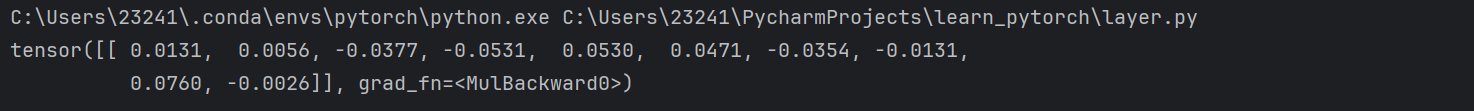
\includegraphics[width = 16cm]{19}
	
	\subsection{使用批归一化}
	批归一化 nn.BatchNorm1d(20) 对每个批次的数据进行归一化,使其具有相同的均值和方差,加速收敛并提高模型的泛化能力
	
	\begin{lstlisting}
import torch
import torch.nn as nn

# 定义一个简单的网络带批归一化
class SimpleNetWithBN(nn.Module):
    def __init__(self):
        super(SimpleNetWithBN, self).__init__()
        self.fc1 = nn.Linear(10, 20)
        self.bn1 = nn.BatchNorm1d(20)
        self.fc2 = nn.Linear(20, 1)

    def forward(self, x):
        x = self.bn1(self.fc1(x))
        return self.fc2(x)

# 实例化模型并使用
x = torch.randn(5, 10)
model = SimpleNetWithBN()
output = model(x)
print(output)
    \end{lstlisting}
	
	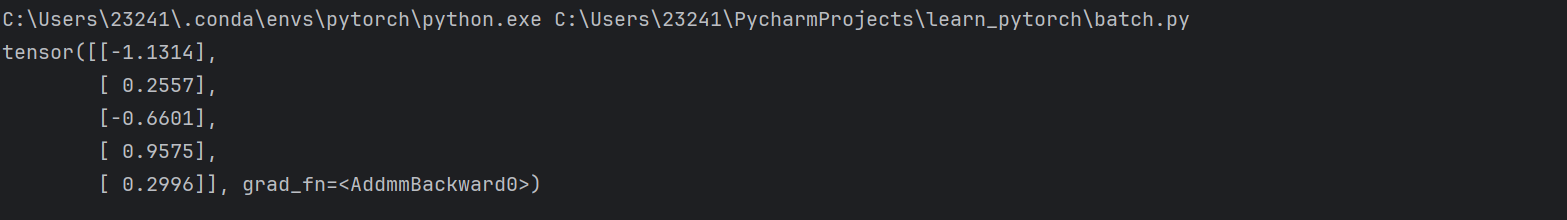
\includegraphics[width = 16cm]{20}

	\section{实验收获与感悟}
	通过学习调试与性能分析、元编程、大杂烩以及 PyTorch 的使用,我对编程有了更深入的理解。在调试和性能分析方面,不同工具的灵活使用让我能够高效定位问题,特别是在复杂系统中,通过日志、性能剖析工具等方法,我更能够系统化地分析代码性能瓶颈,并优化程序的执行效率。\\
	\indent 元编程的学习则让我体会到代码的自动化与灵活性。构建系统、依赖管理、自动化测试等技术不仅提升了工作效率,也让代码更加可扩展和可靠。在大型项目中,自动化工具的应用能够显著减少人为错误,同时大大加速开发和迭代过程。\\
	\indent 大杂烩中Markdown的简洁与高效性在文档编写和知识分享中非常有用,我可以用简单的语法快速创建结构化的文档,并在多个平台上无缝使用它,增强了工作流程的连贯性和效率。\\
	\indent PyTorch 作为深度学习框架的灵活性与强大生态让我能够更方便地构建、调试和优化模型。特别是 GPU 加速与性能优化方面,通过学习分布式训练和混合精度训练技术,我认识到硬件资源的高效利用对大型模型训练的关键作用。总体来说,这些学习经验不仅丰富了我的技术储备,还让我在编程、调试、优化与自动化等方面的能力得到了系统提升。\\
	
	Github仓库链接:\url{https://github.com/xwelkin/lab.git}
	
\end{sloppypar}
\end{document}